\documentclass{article}



\usepackage{arxiv}

\usepackage[utf8]{inputenc} % allow utf-8 input
\usepackage[T1]{fontenc}    % use 8-bit T1 fonts
\usepackage{hyperref}       % hyperlinks
\usepackage{url}            % simple URL typesetting
\usepackage{booktabs}       % professional-quality tables
\usepackage{amsfonts}       % blackboard math symbols
\usepackage{nicefrac}       % compact symbols for 1/2, etc.
\usepackage{microtype}      % microtypography
\usepackage{lipsum}		% Can be removed after putting your text content
\usepackage{graphicx}
\usepackage{natbib}
\usepackage{doi}
\usepackage{float}

\usepackage{xcolor}
\hypersetup{
	colorlinks,
	linkcolor={red!50!black},
	citecolor={blue!50!black},
	urlcolor={blue!80!black}
}

\title{Scalable Computing Project 3 - P2P Computing with NDN for Hospital Patient Data Exchange}


\date{November, 2023}


\author{
		{
\includegraphics[scale=0.2]{star.png}\hspace{1mm}
	Anupal Mishra	                     }\\
	<ID>          \\
	\texttt{shortname@tcd.ie}            \\
	\And
	{
\includegraphics[scale=0.2]{star.png}\hspace{1mm}
	Noêl Mathis	                 	 }\\
	23337722                          \\
	\texttt{mathisn@tcd.ie}            \\
	\And
	{
\includegraphics[scale=0.2]{star.png}\hspace{1mm}
	Nupur Rathod		             	 }\\
	<ID>                                  \\
	\texttt{shortname@tcd.ie}            \\
	\And
	{
\includegraphics[scale=0.2]{star.png}\hspace{1mm}
	Frason Francis      	         	 }\\
	<ID>                                  \\
	\texttt{shortname@tcd.ie}            \\
}


\begin{document}
	\maketitle
	\section{Scenario and Ideas for Implementation}
	Our scenario addresses the problem of transmitting medical data in real time in hospitals. In such a facility, nurses and doctors may want to have a real-time overview of their patients current medical data. They could, for example, use an app on a tablet as they move around the hospital. Traditionally, this would probably be done via the internet and WiFi. This could cause several problems. One is that WiFi is open to interception and intrusion and another is that modern technologies such as WiFi 6 use frequencies that cause high levels of radiation, which is not conducive in a health-sensitive environment. In addition, hospitals are usually large buildings with multiple wings, which means that the networks need to cover a large area. Finally, a big advantage of NDN could be that changing devices that generate medical data is not really significant, as their data names can start with a prefix, e.g. the patient ID, instead of having a new IP, which could cause additional hassle.
	\begin{figure}[H]
		\centering
		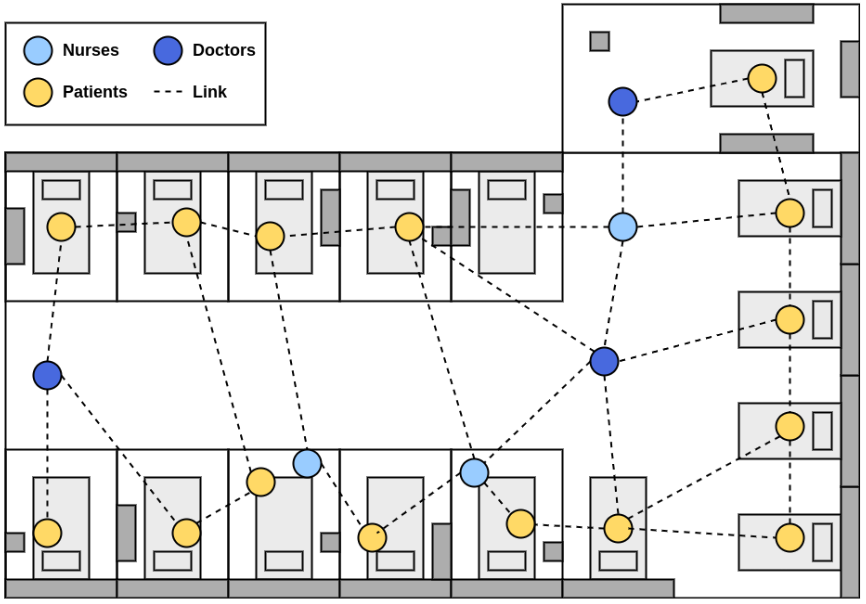
\includegraphics[scale=0.4]{media/scenario.png}
		\caption{Scenario}
		\label{fig:scenario_graphic}
	\end{figure}
	Figure~\ref{fig:scenario_graphic} visualises an example of our scenario. The blue dots show nurses and doctors who are in the environment, while the patients wearing some kind of medical device are mostly in their rooms in this example. The data is then transferred to the nurses/doctors via links. A data transmission may also require multiple hops across other nodes, which may be both patient and staff devices, to reach the consumer. As all devices on this network are owned by one organisation, in this case the hospital, hop-to-hop encryption may be sufficient. A key issue is to ensure that no untrusted devices can enter the network, which is covered later in this report.
	\section{Implementation Details}
	\subsection{Physical Layer and KNN}
	\begin{figure}[H]
		\centering
		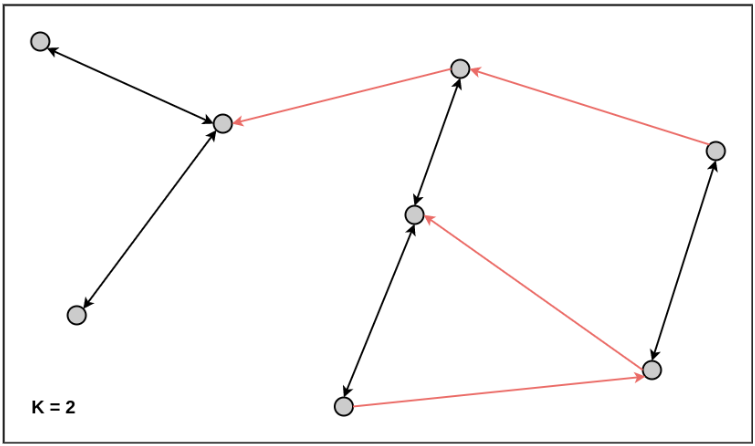
\includegraphics[scale=0.4]{media/knn.png}
		\caption{KNN to Simulate Physical Space}
		\label{fig:knn}
	\end{figure}
	The figure above shows a simple simulation of our network. To simulate a physical space, our nodes are randomly distributed in a 2d grid. A seed for the Python random library is used on both pis to ensure that all nodes are distributed similarly. Then each pi later uses processes to start half the nodes. Moreover, knn is used to determine a fixed number of nearest neighbours. Each node can only communicate with these neighbours. This leads to the problem that is symbolised by the red arrows, which can sometimes lead to one-way connections. However, this is not realistic, as in a real P2P network hello messages would probably simply be passed to all nodes within broadcast range. Here this was solved by hello acknowledgements, how exactly will be explained in the chapter following this one.\\
	Each node furthermore consists of Sensors to gather data, the NDN part which is responsible for fullfilling all obligations a node has in regards to participating in NDN networking and links which is required due to the way TCP/IP and the physical layer is used. Links consists of the IP-addresses and ports of the k-nearest neighbours.
	\begin{figure}[H]
		\centering
		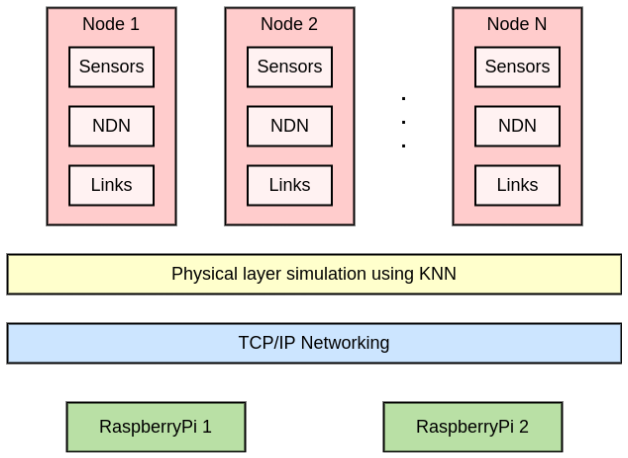
\includegraphics[scale=0.4]{media/network_layers.png}
		\caption{Network Architecture}
		\label{fig:network_layers}
	\end{figure}
	In general our network architecture is built as it is displayed in~\ref{fig:network_layers}. We continue to use TCP/IP networking to send the data. However, our simulation, which in turn is based on the previously explained physical layer simulation, is independent of this and should be seen as an abstraction. TCP/IP had to be used due to the limitations of this task in terms of time and technology.
	\subsection{Dynamic Neighbour Discovery}
	For dynamic discovery, each node has a life cycle. Within this cycle, messages are sent to all neighbours at a fixed time interval. To recognise dead nodes at the same time, the fib has a hello counter next to the IP and port. This is decremented during the life cycle.
	\begin{figure}[H]
		\centering
		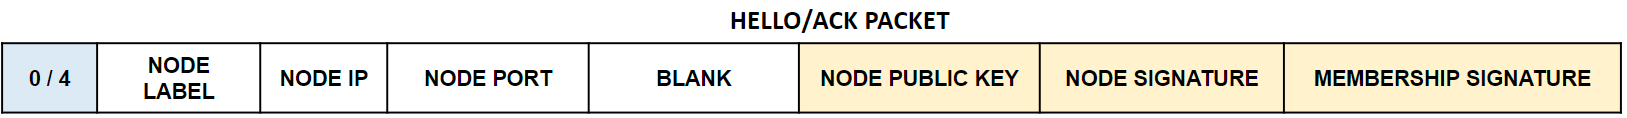
\includegraphics[scale=0.4]{media/hello_ack_package.png}
		\caption{Hello Package Structure}
		\label{fig:hello_ack_package}
	\end{figure}
	In addition, each message contains the sender's public key, his signature and a membership signature. The exact meaning of these components is explained in chapter~\ref{TODO}. Node label is used to identify each node within the FIB table.\\
	To solve the problem of one-directional connections between nodes we introduced hello acknowledgment messages. Each time a node receives a hello message it sends back a hallo-ack message. The receiver then treats this in the exact same way as a normal hello message would have been treated, with the only difference being that no hello-acks are sent for hello-acks since that would create infinite loops.\\
	Hello-ack and hello packages are distinguished by different identifiers which can be seen in the blue box of the package structure. Zero is a hello message and four is a hello-ack message.
	\subsection{...}
	\section{Demo}
	....
	\subsection{Web-UI}
	We also developed a web UI that could be used as a monitoring tool in the long term. Our Python programmes regularly write the status of all nodes to a json file for each pi. The exact structure of this file can be viewed in the code under frontend/ui/src/types/index.ts. The actual json file uses the node keys as keys and the interface NodeState as valuetypes. These two JSONs are then shared with Macneil via our HomeDirectory and made available there via the automatically available web server.\\
	Since React executes http requests in the browser, a small backend was developed for easier handling, which acts as a proxy for the react app. This also aggregates the two state files. These state files are then used to display a graph of the network in the browser. Further details can be loaded by clicking on each node. This can be seen in the following picture:\\
	\begin{figure}[H]
		\centering
		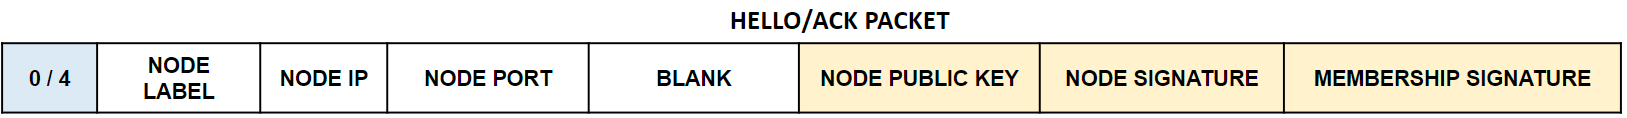
\includegraphics[scale=0.4]{media/hello_ack_package.png}
		\caption{Hello Package Structure}
		\label{fig:hello_ack_package}
	\end{figure}
	Other details like FIB(hello counts, connections to other nodes, etc.) are visualized in the graph. This can be seen in all of the images. The node with the golden border is the node responsible for cross network communication. Finally, the visualisation can be updated by clicking on the corresponding button or by reloading the website. For example, nodes that are offline are displayed in red and connections that no longer exist due to the hello mechanism are no longer displayed. This can be seen in the following figure:
	\begin{figure}[H]
		\centering
		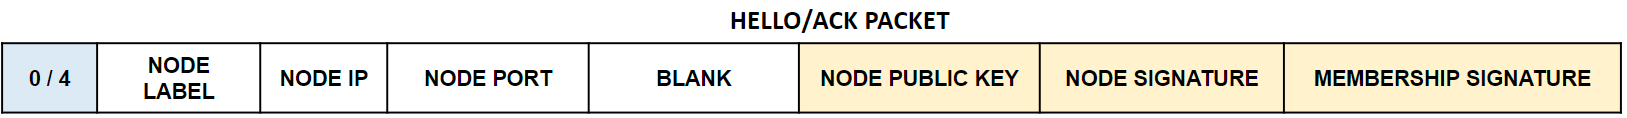
\includegraphics[scale=0.4]{media/hello_ack_package.png}
		\caption{Hello Package Structure}
		\label{fig:hello_ack_package}
	\end{figure}

	\bibliographystyle{unsrtnat}
	\bibliography{references}













%%% Uncomment this line and comment out the ``thebibliography'' section below to use the external .bib file (using bibtex) .


%%% Uncomment this section and comment out the \bibliography{references} line above to use inline references.
% \begin{thebibliography}{1}

% 	\bibitem{kour2014real}
% 	George Kour and Raid Saabne.
% 	\newblock Real-time segmentation of on-line handwritten arabic script.
% 	\newblock In {\em Frontiers in Handwriting Recognition (ICFHR), 2014 14th
% 			International Conference on}, pages 417--422. IEEE, 2014.

% 	\bibitem{kour2014fast}
% 	George Kour and Raid Saabne.
% 	\newblock Fast classification of handwritten on-line arabic characters.
% 	\newblock In {\em Soft Computing and Pattern Recognition (SoCPaR), 2014 6th
% 			International Conference of}, pages 312--318. IEEE, 2014.

% 	\bibitem{hadash2018estimate}
% 	Guy Hadash, Einat Kermany, Boaz Carmeli, Ofer Lavi, George Kour, and Alon
% 	Jacovi.
% 	\newblock Estimate and replace: A novel approach to integrating deep neural
% 	networks with existing applications.
% 	\newblock {\em arXiv preprint arXiv:1804.09028}, 2018.

% \end{thebibliography}


\end{document}
